\begin{figure}[H]
    \centering
    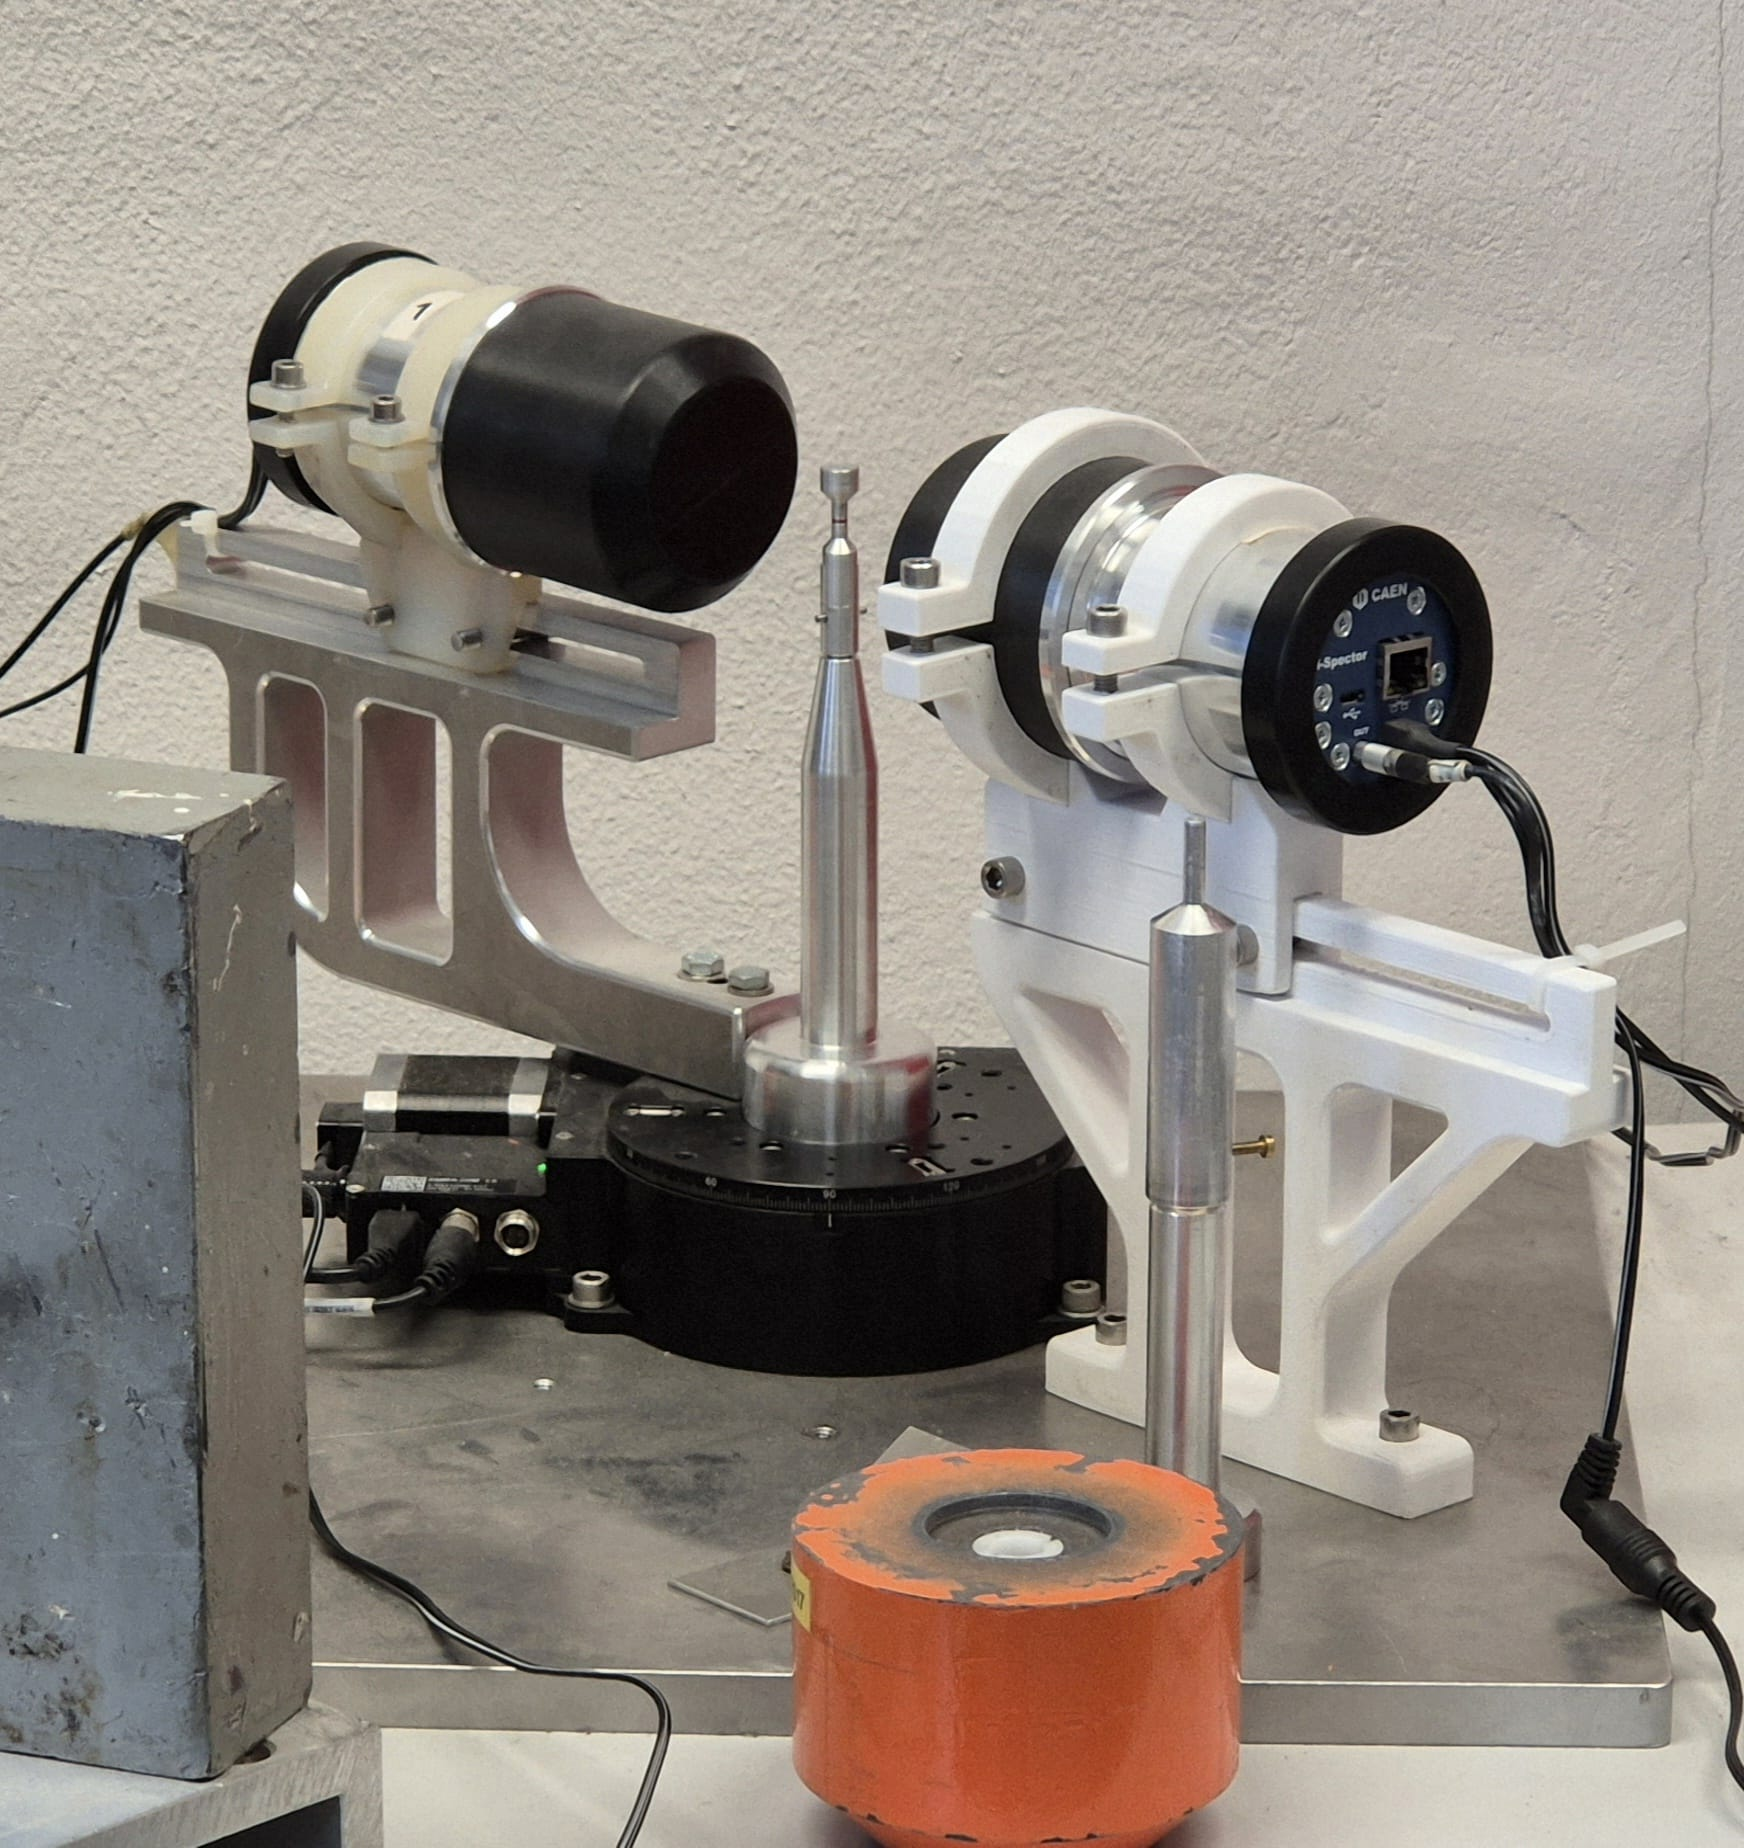
\includegraphics[width=0.5\linewidth]{../Images/Setup.jpeg}
    \caption{Image of the Experimental Setup. The two detectors sit on opposite sides of the $^{60}$Co source. The detector nearer to the camera was kept stationary in the experiment, while the one further away was rotated; at the moment (and for the calibration part of the experiment) the angle between them is $180\degree$. The orange container in the front is the container for the radioactive source.}
    \label{fig:setup}
\end{figure}

At the beginning of the experiment, the movable detector was set $180\degree$ across from the stationary detector, directly opposite it. It was kept in this position for the first part of the experiment (the steps detailed in the next subsection).\\

The first thing we did was measure the distance of the source from the two detectors. Since the source was placed in between the two, we did this by measuring the distance between the two detectors and halving it. This distance was measured to be $90\pm1\,\text{mm}$, which halves to give us a distance between the source and the detectors of $45\pm0.5\,\text{mm}$. However, both detectors had a cap of thickness $5\,$mm, meaning the actual distance between the source and each detector was $50\pm0.5\,$mm.\\
